% Incremental memory management, transcribed from the original figure.
% Hollow/filled circles are instruction head bits, not opcode characters.
\resizebox{0.78\textwidth}{!}{%
  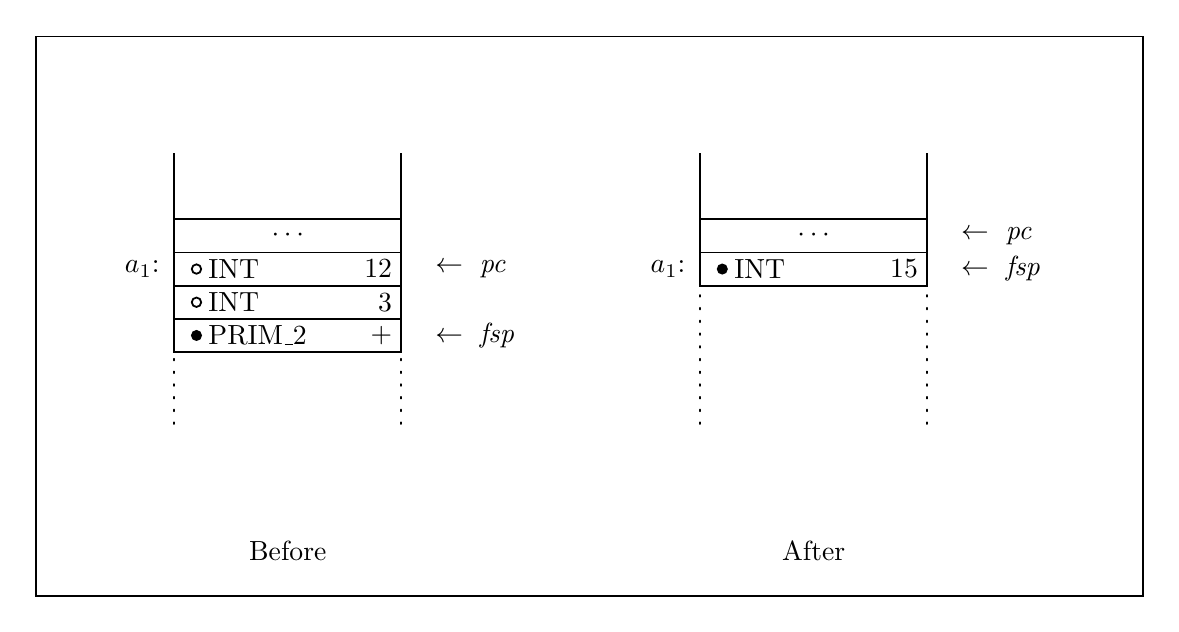
\begin{tikzpicture}[x=1pt,y=1pt,line width=0.65pt,
    font=\normalsize,inner sep=0pt,
    omitted/.style={dash pattern=on 0.6pt off 4pt,line cap=round}]
    \path[use as bounding box] (-3,-3) rectangle (403,205.2214);
    \draw (0,0) rectangle (400,202);
    \foreach \x in {50,240} {
      \draw (\x,136) -- (\x,160);
      \draw (\x+82,136) -- (\x+82,160);
      \draw (\x,112) rectangle (\x+82,136);
      \draw (\x,124) -- (\x+82,124);
      \node at (\x+41,130) {\(\cdots\)};
      \node[anchor=west] at (\x+12,118) {INT};
      \node[anchor=east] at (\x-5,118) {\(a_1\):};
    }
    \draw (50,88) rectangle (132,112);
    \draw (50,100) -- (132,100);
    \draw (58,118) circle (1.7pt);
    \draw (58,106) circle (1.7pt);
    \fill (58,94) circle (2pt);
    \node[anchor=west] at (62,106) {INT};
    \node[anchor=west] at (62,94) {PRIM\_2};
    \node[anchor=east] at (129,118) {12};
    \node[anchor=east] at (129,106) {3};
    \node[anchor=east] at (129,94) {\(+\)};
    \draw[omitted] (50,62) -- (50,88);
    \draw[omitted] (132,62) -- (132,88);
    \node[anchor=west] at (144,118) {\(\leftarrow\ \mathit{pc}\)};
    \node[anchor=west] at (144,94) {\(\leftarrow\ \mathit{fsp}\)};
    \fill (248,118) circle (2pt);
    \node[anchor=east] at (319,118) {15};
    \draw[omitted] (240,62) -- (240,112);
    \draw[omitted] (322,62) -- (322,112);
    \node[anchor=west] at (334,130) {\(\leftarrow\ \mathit{pc}\)};
    \node[anchor=west] at (334,118) {\(\leftarrow\ \mathit{fsp}\)};
    \node at (91,16) {Before};
    \node at (281,16) {After};
  \end{tikzpicture}%
}
